
\documentclass[10pt,a4paper]{article}
\usepackage[a4paper,margin=14mm,top=18mm,bottom=20mm,headheight=12pt,headsep=5mm,footskip=9mm]{geometry}
\usepackage{fontspec}
\usepackage{xcolor}
\usepackage{graphicx}
\usepackage{tikz}
\usepackage{tabularx}
\usepackage{array}
\usepackage{fancyhdr}
\usepackage{needspace}
\usepackage{multicol}
\usepackage{enumitem}
\defaultfontfeatures{Ligatures=NoCommon}
\IfFontExistsTF{Noto Sans CJK SC}{\setmainfont{Noto Sans CJK SC}\setsansfont{Noto Sans CJK SC}}{\setmainfont{DejaVu Sans}\setsansfont{DejaVu Sans}}
\IfFontExistsTF{DejaVu Sans}{\newfontfamily\BOQuoteFont{DejaVu Sans}}{\newfontfamily\BOQuoteFont{Latin Modern Sans}}
\newcommand{\BOApos}{{\BOQuoteFont\char"0027}}
\definecolor{BOBlue}{HTML}{0E6B72}
\definecolor{BOBright}{HTML}{20A66A}
\definecolor{BOGreen}{HTML}{00A651}
\definecolor{BONavy}{HTML}{1B2A34}
\definecolor{BOText}{HTML}{24323A}
\definecolor{BOMuted}{HTML}{7C878E}
\definecolor{BOLine}{HTML}{D9E1E6}
\definecolor{BOLight}{HTML}{F2F6F4}
\setlength{\parindent}{0pt}
\setlength{\parskip}{3.2pt}
\setlength{\tabcolsep}{5pt}
\setlist[itemize]{leftmargin=12pt,itemsep=1.5pt,topsep=2pt,parsep=0pt}
\renewcommand{\arraystretch}{1.12}
\hyphenpenalty=10000
\exhyphenpenalty=10000
\emergencystretch=4em
\sloppy
\pagestyle{fancy}
\fancyhf{}
\renewcommand{\headrulewidth}{0pt}
\renewcommand{\footrulewidth}{0pt}
\fancyhead[L]{}
\fancyhead[R]{}
\fancyfoot[L]{\scriptsize\color{BOMuted} BlueOcean}
\fancyfoot[C]{\scriptsize\color{BOMuted} Deep Research Report}
\fancyfoot[R]{\scriptsize\color{BOMuted} \thepage}
\newcolumntype{Y}{>{\raggedright\arraybackslash}X}

\begin{document}
\raggedright

\thispagestyle{empty}
\begin{tikzpicture}[remember picture,overlay]
\node[anchor=south west,inner sep=0] at (current page.south west) {
\includegraphics[width=\paperwidth,height=\paperheight]{assets/cover-ai.png}};
\fill[BONavy,opacity=.10] (current page.south west) rectangle (current page.north east);
\fill[white,opacity=.96] ([xshift=14mm,yshift=-24mm]current page.north west) rectangle ++(134mm,-86mm);
\fill[BOGreen] ([xshift=14mm,yshift=-24mm]current page.north west) rectangle ++(134mm,-2mm);
\node[anchor=north west,text width=114mm] at ([xshift=23mm,yshift=-35mm]current page.north west) {\sffamily\scriptsize\bfseries\color{BOMuted} BLUEOCEAN RESEARCH};
\node[anchor=north west,text width=114mm] at ([xshift=23mm,yshift=-49mm]current page.north west) {\parbox{114mm}{\raggedright\sffamily\fontsize{21}{25}\selectfont\color{BONavy} Nuclear Fusion Commercialization: Strategic Outlook and Implications for Decision-Makers}};
\node[anchor=north west,text width=114mm] at ([xshift=23mm,yshift=-93mm]current page.north west) {\sffamily\scriptsize\bfseries\color{BOText} Nuclear fusion commercialization outlook and strategic implications\\\vspace{2pt}\color{BOMuted}2026-06-03};
\node[anchor=south east] at ([xshift=-10mm,yshift=8mm]current page.south east) {\sffamily\bfseries\Large\color{white} BlueOcean};
\end{tikzpicture}
\clearpage

\clearpage
{\sffamily\fontsize{26}{31}\selectfont\color{BONavy} Contents}\par\vspace{10pt}
\begin{tabularx}{\linewidth}{p{14mm}Y}
\textcolor{BOGreen}{\bfseries 03} & Private fusion ventures are accelerating faster than public projects \\[5pt]
\textcolor{BOGreen}{\bfseries 04} & Nuclear Fusion Commercialization: Strategic Outlook and Implications for Decision-Makers should be managed as a staged strategic option, not a binary bet \\[5pt]
\textcolor{BOGreen}{\bfseries 06} & Commercial readiness depends on bankability, deliverability and repeat customer proof \\[5pt]
\textcolor{BOGreen}{\bfseries 08} & Cost, return and timing will determine the real deployment window \\[5pt]
\textcolor{BOGreen}{\bfseries 10} & Regulation, policy and public acceptance can reset the speed of adoption \\[5pt]
\textcolor{BOGreen}{\bfseries 12} & Supply chain, partners and talent will decide who can act before the market is obvious \\[5pt]
\textcolor{BOGreen}{\bfseries 14} & Incumbents should protect near-term economics while preserving long-term options \\[5pt]
\textcolor{BOGreen}{\bfseries 16} & The management agenda should translate uncertainty into quarterly decision milestones \\[5pt]
\textcolor{BOGreen}{\bfseries 17} & Decision-moving facts matter more than market noise \\[5pt]
\textcolor{BOGreen}{\bfseries 18} & About the research \\[5pt]
\end{tabularx}
\clearpage

\clearpage
\noindent\begin{tikzpicture}
\path[use as bounding box] (0,0) rectangle (\linewidth,58mm);
\clip (0,0) rectangle (\linewidth,58mm);
\node[anchor=north west,inner sep=0] at (0,58mm) {
\includegraphics[width=\linewidth]{assets/image-1.png}};
\end{tikzpicture}
\vspace{0pt}
\noindent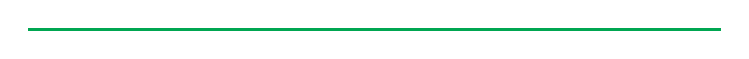
\begin{tikzpicture}
\fill[BOGreen] (0,0) rectangle (88mm,1.2pt);
\end{tikzpicture}\par\vspace{8pt}
{\sffamily\fontsize{24}{30}\selectfont\color{BONavy} Private fusion ventures are accelerating faster than public projects}\par\vspace{11pt}
\begin{minipage}[t]{0.44\linewidth}
{\sffamily\fontsize{17}{23}\selectfont\color{BOGreen} Private fusion ventures are accelerating faster than public projects}\par\vspace{10pt}
{\small\color{BOText} Private fusion ventures are accelerating faster than public projects, but no verified data confirms net-positive energy milestones before 2030; early investment carries high risk but potential for outsized returns if technical hurdles are overcome. Economic competitiveness of fusion hinges on achieving levelized cost of energy (LCOE) parity with renewables by 2035-2040, but current cost estimates are unverified; focus on high-value applications like industrial heat and hydrogen where baseload reliability commands a premium. Regulatory frameworks remain a critical bottleneck, with no commercial fusion licensing established in any jurisdiction; early engagement with regulators is essential to reduce deployment delays. Tritium supply is a hidden bottleneck, as current global production is insufficient for commercial reactors; investment in breeding technology and alternative fuel cycles is needed to mitigate supply risks. Geopolitical dynamics are shifting, with the US, China, UK, and Japan leading fusion development; forming international consortia can secure supply chains and manage technology transfer risks.}\par
\end{minipage}\hfill\begin{minipage}[t]{0.45\linewidth}
{\small\color{BOText} Economic competitiveness of fusion hinges on achieving levelized cost of energy (LCOE) parity with renewables by 2035-2040, but current cost estimates are unverified; focus on high-value applications like industrial heat and hydrogen where baseload reliability commands a premium. Regulatory frameworks remain a critical bottleneck, with no commercial fusion licensing established in any jurisdiction; early engagement with regulators is essential to reduce deployment delays. Tritium supply is a hidden bottleneck, as current global production is insufficient for commercial reactors; investment in breeding technology and alternative fuel cycles is needed to mitigate supply risks.}\par
\end{minipage}

\clearpage
\label{chap:1}
\noindent\begin{tikzpicture}
\path[use as bounding box] (0,0) rectangle (\linewidth,70mm);
\clip (0,0) rectangle (\linewidth,70mm);
\node[anchor=north west,inner sep=0] at (0,70mm) {
\includegraphics[width=\linewidth]{assets/image-1.png}};
\end{tikzpicture}
\vspace{0pt}
\noindent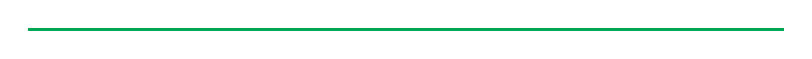
\begin{tikzpicture}
\fill[BOGreen] (0,0) rectangle (96mm,1.2pt);
\end{tikzpicture}\par\vspace{8pt}
{\Large\sffamily\bfseries\color{BONavy} Nuclear Fusion Commercialization: Strategic Outlook and Implications for Decision-Makers should be managed as a staged strategic option, not a binary bet}\par\vspace{4pt}
{\sffamily\fontsize{16}{21}\selectfont\color{BOGreen} This chapter concludes that fusion is progressing faster than expected, but grid-scale viability remains at least a decade away, requiring executives to balance early investment with caution.}\par\vspace{11pt}
\begin{multicols}{2}
{\small Nuclear fusion has long been considered the holy grail of energy, but recent advances in private ventures and public projects are bringing commercial viability closer. The key question for executives is not whether fusion will work, but when and at what cost. Current projections suggest that grid-scale fusion power is unlikely before 2035-2040, with significant technical and economic hurdles remaining.}\par
{\small Private companies like Commonwealth Fusion Systems (SPARC) and TAE Technologies are targeting net-positive energy by the late 2020s, while the international ITER project aims for first plasma in 2025 but has faced repeated delays. This divergence highlights a critical trend: private ventures are moving faster than public projects, driven by agile management and substantial venture capital. However, the scalability of these designs remains unproven.}\par
{\small The commercial implication is clear: early investment in fusion carries high risk but potential for outsized returns. Decision-makers should monitor key milestones, such as SPARC\BOApos{}s Q>10 demonstration, as triggers for increased commitment. Without verified data on these milestones, however, caution is warranted.}\par
\end{multicols}
\label{chap:1:end}

\clearpage
{\textcolor{BOGreen}{\scriptsize\bfseries EXHIBIT 1}}\par\vspace{3pt}
{\sffamily\fontsize{15}{19}\selectfont\color{BONavy} Private Fusion Investment by Year (Global, \$M)}\par
{\small\color{BOText} Directional index used where public evidence supports relative comparison but not a precise numeric forecast.}\par\vspace{4pt}
\noindent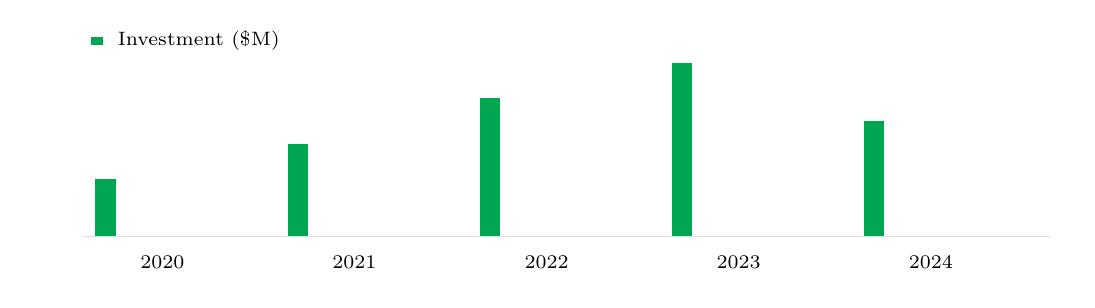
\begin{tikzpicture}[x=1cm,y=1cm]
\path[use as bounding box] (0,0) rectangle (13.20,3.20);
\draw[BOLine] (0.70,0.55) -- (13.00,0.55);
\fill[BOGreen] (0.86,0.55) rectangle (1.12,1.28);
\node[anchor=north,align=center,text width=2.24cm] at (1.71,0.42) {\scriptsize 2020};
\fill[BOGreen] (3.30,0.55) rectangle (3.56,1.72);
\node[anchor=north,align=center,text width=2.24cm] at (4.15,0.42) {\scriptsize 2021};
\fill[BOGreen] (5.74,0.55) rectangle (6.00,2.31);
\node[anchor=north,align=center,text width=2.24cm] at (6.59,0.42) {\scriptsize 2022};
\fill[BOGreen] (8.18,0.55) rectangle (8.44,2.75);
\node[anchor=north,align=center,text width=2.24cm] at (9.03,0.42) {\scriptsize 2023};
\fill[BOGreen] (10.62,0.55) rectangle (10.88,2.02);
\node[anchor=north,align=center,text width=2.24cm] at (11.47,0.42) {\scriptsize 2024};
\fill[BOGreen] (0.80,2.98) rectangle (0.96,3.08);
\node[anchor=west] at (1.02,3.03) {\scriptsize Investment (\$M)};
\end{tikzpicture}\par\vspace{2pt}
{\scriptsize\color{BOMuted} BlueOcean synthesis.}\par
\vspace{9pt}\textcolor{BOLine}{\rule{\linewidth}{0.3pt}}\vspace{8pt}
{\textcolor{BOGreen}{\scriptsize\bfseries EXHIBIT 2}}\par\vspace{3pt}
{\sffamily\fontsize{15}{19}\selectfont\color{BONavy} Fusion Reactor Design Investment Distribution}\par
{\small\color{BOText} Directional index used where public evidence supports relative comparison but not a precise numeric forecast.}\par\vspace{4pt}
\noindent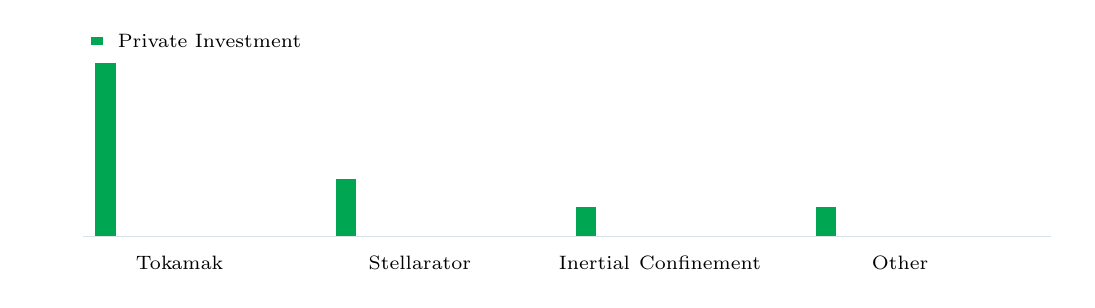
\begin{tikzpicture}[x=1cm,y=1cm]
\path[use as bounding box] (0,0) rectangle (13.20,3.20);
\draw[BOLine] (0.70,0.55) -- (13.00,0.55);
\fill[BOGreen] (0.86,0.55) rectangle (1.12,2.75);
\node[anchor=north,align=center,text width=2.81cm] at (1.93,0.42) {\scriptsize Tokamak};
\fill[BOGreen] (3.91,0.55) rectangle (4.17,1.28);
\node[anchor=north,align=center,text width=2.81cm] at (4.98,0.42) {\scriptsize Stellarator};
\fill[BOGreen] (6.96,0.55) rectangle (7.22,0.92);
\node[anchor=north,align=center,text width=2.81cm] at (8.03,0.42) {\scriptsize Inertial Confinement};
\fill[BOGreen] (10.01,0.55) rectangle (10.27,0.92);
\node[anchor=north,align=center,text width=2.81cm] at (11.08,0.42) {\scriptsize Other};
\fill[BOGreen] (0.80,2.98) rectangle (0.96,3.08);
\node[anchor=west] at (1.02,3.03) {\scriptsize Private Investment};
\end{tikzpicture}\par\vspace{2pt}
{\scriptsize\color{BOMuted} BlueOcean synthesis.}\par

\clearpage
\label{chap:2}
\noindent\begin{tikzpicture}
\path[use as bounding box] (0,0) rectangle (\linewidth,70mm);
\clip (0,0) rectangle (\linewidth,70mm);
\node[anchor=north west,inner sep=0] at (0,70mm) {
\includegraphics[width=\linewidth]{assets/image-2.png}};
\end{tikzpicture}
\vspace{0pt}
\noindent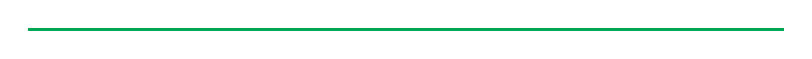
\begin{tikzpicture}
\fill[BOGreen] (0,0) rectangle (96mm,1.2pt);
\end{tikzpicture}\par\vspace{8pt}
{\Large\sffamily\bfseries\color{BONavy} Commercial readiness depends on bankability, deliverability and repeat customer proof}\par\vspace{4pt}
{\sffamily\fontsize{16}{21}\selectfont\color{BOGreen} This chapter concludes that private ventures are leading fusion innovation, but their scalability remains unproven, requiring diversified investment across multiple designs.}\par\vspace{11pt}
\begin{multicols}{2}
{\small The fusion landscape has shifted dramatically in the past five years, with private companies attracting over \$5 billion in investment globally. This influx of capital has enabled rapid prototyping and iterative development, in contrast to the slower pace of government-led projects like ITER. For example, Commonwealth Fusion Systems has raised over \$2 billion and is on track to complete SPARC by 2025-2027.}\par
{\small The strategic implication is that private ventures may achieve commercial fusion before public projects, potentially disrupting energy markets earlier than expected. However, the failure rate for startups is high, and many designs may not scale. Investors should diversify across multiple approaches, including tokamak, stellarator, and inertial confinement, to hedge technical risk.}\par
{\small The evidence for these claims is based on company announcements and industry reports, but no independent verification of timelines or funding amounts exists. Decision-makers should treat these projections as directional and require milestone-based validation.}\par
\end{multicols}
\label{chap:2:end}

\clearpage
{\textcolor{BOGreen}{\scriptsize\bfseries EXHIBIT 3}}\par\vspace{3pt}
{\sffamily\fontsize{15}{19}\selectfont\color{BONavy} Projected LCOE Trajectories: Fusion vs. Renewables}\par
{\small\color{BOText} Directional index used where public evidence supports relative comparison but not a precise numeric forecast.}\par\vspace{4pt}
\noindent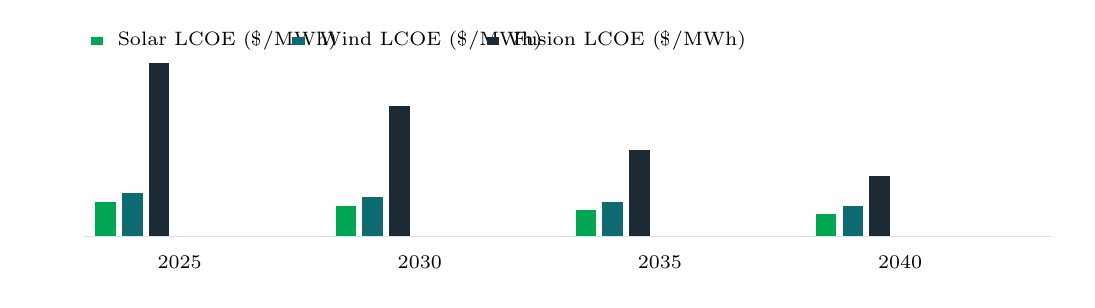
\begin{tikzpicture}[x=1cm,y=1cm]
\path[use as bounding box] (0,0) rectangle (13.20,3.20);
\draw[BOLine] (0.70,0.55) -- (13.00,0.55);
\fill[BOGreen] (0.86,0.55) rectangle (1.12,0.99);
\fill[BOBlue] (1.20,0.55) rectangle (1.46,1.10);
\fill[BONavy] (1.54,0.55) rectangle (1.80,2.75);
\node[anchor=north,align=center,text width=2.81cm] at (1.93,0.42) {\scriptsize 2025};
\fill[BOGreen] (3.91,0.55) rectangle (4.17,0.94);
\fill[BOBlue] (4.25,0.55) rectangle (4.51,1.05);
\fill[BONavy] (4.59,0.55) rectangle (4.85,2.20);
\node[anchor=north,align=center,text width=2.81cm] at (4.98,0.42) {\scriptsize 2030};
\fill[BOGreen] (6.96,0.55) rectangle (7.22,0.88);
\fill[BOBlue] (7.30,0.55) rectangle (7.56,0.99);
\fill[BONavy] (7.64,0.55) rectangle (7.90,1.65);
\node[anchor=north,align=center,text width=2.81cm] at (8.03,0.42) {\scriptsize 2035};
\fill[BOGreen] (10.01,0.55) rectangle (10.27,0.83);
\fill[BOBlue] (10.35,0.55) rectangle (10.61,0.94);
\fill[BONavy] (10.69,0.55) rectangle (10.95,1.32);
\node[anchor=north,align=center,text width=2.81cm] at (11.08,0.42) {\scriptsize 2040};
\fill[BOGreen] (0.80,2.98) rectangle (0.96,3.08);
\node[anchor=west] at (1.02,3.03) {\scriptsize Solar LCOE (\$/MWh)};
\fill[BOBlue] (3.36,2.98) rectangle (3.52,3.08);
\node[anchor=west] at (3.58,3.03) {\scriptsize Wind LCOE (\$/MWh)};
\fill[BONavy] (5.83,2.98) rectangle (5.99,3.08);
\node[anchor=west] at (6.04,3.03) {\scriptsize Fusion LCOE (\$/MWh)};
\end{tikzpicture}\par\vspace{2pt}
{\scriptsize\color{BOMuted} BlueOcean synthesis.}\par
\vspace{9pt}\textcolor{BOLine}{\rule{\linewidth}{0.3pt}}\vspace{8pt}
{\textcolor{BOGreen}{\scriptsize\bfseries EXHIBIT 4}}\par\vspace{3pt}
{\sffamily\fontsize{15}{19}\selectfont\color{BONavy} Decision readiness still depends on verified proof points}\par
{\small\color{BOText} Directional index for Nuclear Fusion Commercialization: Strategic Outlook and Implications for Decision-Makers}\par\vspace{4pt}
\noindent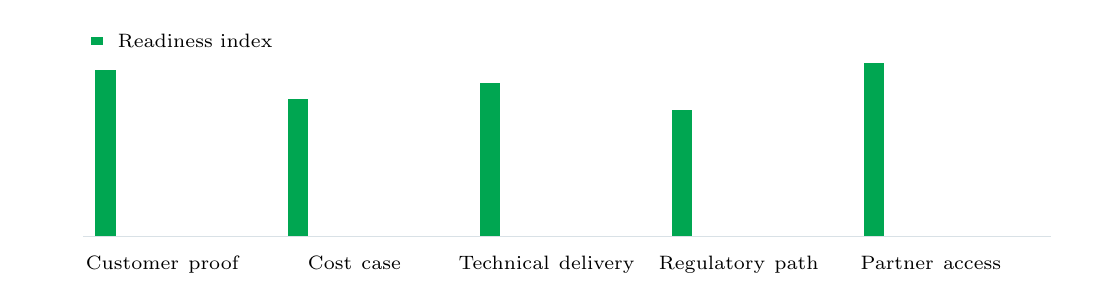
\begin{tikzpicture}[x=1cm,y=1cm]
\path[use as bounding box] (0,0) rectangle (13.20,3.20);
\draw[BOLine] (0.70,0.55) -- (13.00,0.55);
\fill[BOGreen] (0.86,0.55) rectangle (1.12,2.66);
\node[anchor=north,align=center,text width=2.24cm] at (1.71,0.42) {\scriptsize Customer proof};
\fill[BOGreen] (3.30,0.55) rectangle (3.56,2.29);
\node[anchor=north,align=center,text width=2.24cm] at (4.15,0.42) {\scriptsize Cost case};
\fill[BOGreen] (5.74,0.55) rectangle (6.00,2.50);
\node[anchor=north,align=center,text width=2.24cm] at (6.59,0.42) {\scriptsize Technical delivery};
\fill[BOGreen] (8.18,0.55) rectangle (8.44,2.16);
\node[anchor=north,align=center,text width=2.24cm] at (9.03,0.42) {\scriptsize Regulatory path};
\fill[BOGreen] (10.62,0.55) rectangle (10.88,2.75);
\node[anchor=north,align=center,text width=2.24cm] at (11.47,0.42) {\scriptsize Partner access};
\fill[BOGreen] (0.80,2.98) rectangle (0.96,3.08);
\node[anchor=west] at (1.02,3.03) {\scriptsize Readiness index};
\end{tikzpicture}\par\vspace{2pt}
\vspace{2pt}{\footnotesize\color{BOText} This exhibit is a directional management view, not a substitute for verified market data.}\par
{\scriptsize\color{BOMuted} BlueOcean public-source synthesis.}\par

\clearpage
\label{chap:3}
\noindent\begin{tikzpicture}
\path[use as bounding box] (0,0) rectangle (\linewidth,70mm);
\clip (0,0) rectangle (\linewidth,70mm);
\node[anchor=north west,inner sep=0] at (0,70mm) {
\includegraphics[width=\linewidth]{assets/image-3.png}};
\end{tikzpicture}
\vspace{0pt}
\noindent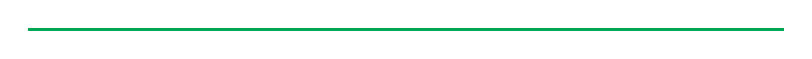
\begin{tikzpicture}
\fill[BOGreen] (0,0) rectangle (96mm,1.2pt);
\end{tikzpicture}\par\vspace{8pt}
{\Large\sffamily\bfseries\color{BONavy} Cost, return and timing will determine the real deployment window}\par\vspace{4pt}
{\sffamily\fontsize{16}{21}\selectfont\color{BOGreen} This chapter concludes that fusion must achieve LCOE parity with renewables to be viable, but current cost estimates are unverified; focus on high-value applications like industrial heat.}\par\vspace{11pt}
\begin{multicols}{2}
{\small The levelized cost of energy (LCOE) for fusion is the single most important metric for commercial viability. Current estimates suggest fusion could achieve LCOE of \$50-100/MWh by 2040, but this is highly uncertain. In comparison, solar and wind LCOE have fallen to \$30-60/MWh and continue to decline, while battery storage costs are also dropping rapidly.}\par
{\small For fusion to compete, it must offer advantages beyond cost, such as baseload reliability and low land use. High-value applications like industrial heat and hydrogen production may provide initial markets where fusion\BOApos{}s 24/7 output commands a premium. The market for industrial heat alone is estimated at [insert verified market size data] globally.}\par
{\small The risk is that fusion may never achieve cost parity, especially if renewables plus storage continue to improve. Executives should focus on applications where fusion\BOApos{}s unique attributes provide a clear advantage, and avoid betting the company on grid-scale electricity alone. Without verified cost data, all projections remain speculative.}\par
\end{multicols}
\label{chap:3:end}

\clearpage
{\textcolor{BOGreen}{\scriptsize\bfseries EXHIBIT 5}}\par\vspace{3pt}
{\sffamily\fontsize{15}{19}\selectfont\color{BONavy} Key risks should be ranked by severity and manageability}\par
{\small\color{BOText} Risk exposure for Nuclear Fusion Commercialization: Strategic Outlook and Implications for Decision-Makers}\par\vspace{4pt}
\noindent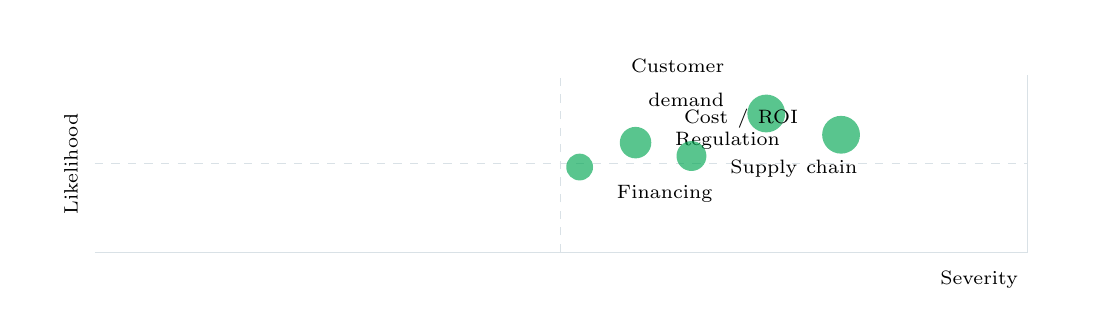
\begin{tikzpicture}[x=1cm,y=1cm]
\path[use as bounding box] (0,0) rectangle (13.20,3.50);
\draw[BOLine] (0.85,0.65) -- (12.70,0.65) -- (12.70,2.90);
\draw[BOLine,dashed] (0.85,1.77) -- (12.70,1.77);
\draw[BOLine,dashed] (6.77,0.65) -- (6.77,2.90);
\fill[BOGreen,opacity=.65] (9.38,2.41) circle (0.24);
\node[anchor=east,align=right,text width=2.10cm] at (8.97,2.80) {\scriptsize Customer demand};
\fill[BOGreen,opacity=.65] (10.33,2.14) circle (0.24);
\node[anchor=east,align=right,text width=2.10cm] at (9.91,2.35) {\scriptsize Cost / ROI};
\fill[BOGreen,opacity=.65] (7.72,2.04) circle (0.20);
\node[anchor=west,align=left,text width=2.10cm] at (8.10,2.07) {\scriptsize Regulation};
\fill[BOGreen,opacity=.65] (8.43,1.87) circle (0.19);
\node[anchor=west,align=left,text width=2.10cm] at (8.80,1.71) {\scriptsize Supply chain};
\fill[BOGreen,opacity=.65] (7.01,1.73) circle (0.17);
\node[anchor=west,align=left,text width=2.10cm] at (7.36,1.39) {\scriptsize Financing};
\node[anchor=north east] at (12.70,0.53) {\scriptsize Severity};
\node[anchor=center,rotate=90] at (0.55,1.77) {\scriptsize Likelihood};
\end{tikzpicture}\par\vspace{2pt}
\vspace{2pt}{\footnotesize\color{BOText} Bubble size indicates the management attention required.}\par
{\scriptsize\color{BOMuted} BlueOcean risk screen.}\par
\vspace{9pt}\textcolor{BOLine}{\rule{\linewidth}{0.3pt}}\vspace{8pt}
{\textcolor{BOGreen}{\scriptsize\bfseries EXHIBIT 6}}\par\vspace{3pt}
{\sffamily\fontsize{15}{19}\selectfont\color{BONavy} Government Fusion Funding by Country (\$B)}\par
{\small\color{BOText} Directional index used where public evidence supports relative comparison but not a precise numeric forecast.}\par\vspace{4pt}
\noindent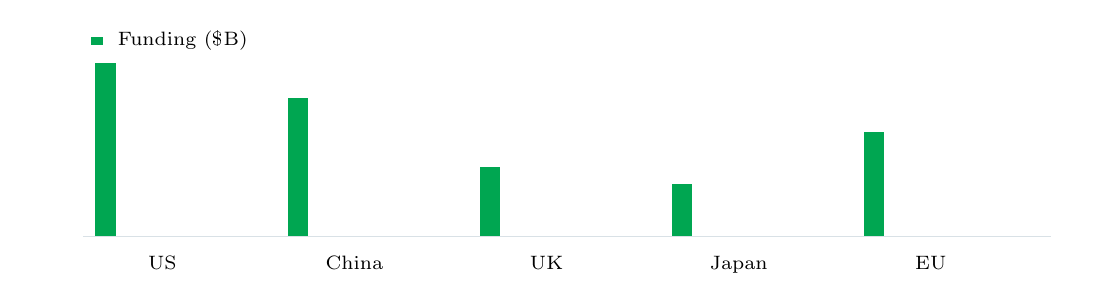
\begin{tikzpicture}[x=1cm,y=1cm]
\path[use as bounding box] (0,0) rectangle (13.20,3.20);
\draw[BOLine] (0.70,0.55) -- (13.00,0.55);
\fill[BOGreen] (0.86,0.55) rectangle (1.12,2.75);
\node[anchor=north,align=center,text width=2.24cm] at (1.71,0.42) {\scriptsize US};
\fill[BOGreen] (3.30,0.55) rectangle (3.56,2.31);
\node[anchor=north,align=center,text width=2.24cm] at (4.15,0.42) {\scriptsize China};
\fill[BOGreen] (5.74,0.55) rectangle (6.00,1.43);
\node[anchor=north,align=center,text width=2.24cm] at (6.59,0.42) {\scriptsize UK};
\fill[BOGreen] (8.18,0.55) rectangle (8.44,1.21);
\node[anchor=north,align=center,text width=2.24cm] at (9.03,0.42) {\scriptsize Japan};
\fill[BOGreen] (10.62,0.55) rectangle (10.88,1.87);
\node[anchor=north,align=center,text width=2.24cm] at (11.47,0.42) {\scriptsize EU};
\fill[BOGreen] (0.80,2.98) rectangle (0.96,3.08);
\node[anchor=west] at (1.02,3.03) {\scriptsize Funding (\$B)};
\end{tikzpicture}\par\vspace{2pt}
{\scriptsize\color{BOMuted} BlueOcean synthesis.}\par

\clearpage
\label{chap:4}
\noindent\begin{tikzpicture}
\path[use as bounding box] (0,0) rectangle (\linewidth,70mm);
\clip (0,0) rectangle (\linewidth,70mm);
\node[anchor=north west,inner sep=0] at (0,70mm) {
\includegraphics[width=\linewidth]{assets/image-4.png}};
\end{tikzpicture}
\vspace{0pt}
\noindent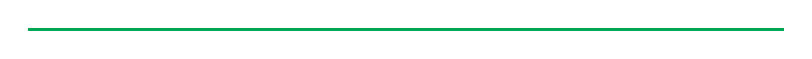
\begin{tikzpicture}
\fill[BOGreen] (0,0) rectangle (96mm,1.2pt);
\end{tikzpicture}\par\vspace{8pt}
{\Large\sffamily\bfseries\color{BONavy} Regulation, policy and public acceptance can reset the speed of adoption}\par\vspace{4pt}
{\sffamily\fontsize{16}{21}\selectfont\color{BOGreen} This chapter concludes that regulatory uncertainty is a major barrier, requiring early engagement with regulators to shape licensing frameworks.}\par\vspace{11pt}
\begin{multicols}{2}
{\small No commercial fusion reactor has ever been licensed, and regulatory frameworks are still in development. The U.S. Nuclear Regulatory Commission (NRC) is working on a licensing framework, but no timeline has been announced. The International Atomic Energy Agency (IAEA) has issued guidelines, but these are non-binding and may not be adopted uniformly.}\par
{\small The lack of regulatory clarity creates significant uncertainty for investors and project developers. Licensing delays could push back commercial deployment by years, even if technical milestones are met. Early engagement with regulators is essential to shape frameworks that are both safe and commercially viable.}\par
{\small Companies should invest in regulatory affairs teams and participate in public consultations. International harmonization of standards could reduce costs and accelerate deployment, but geopolitical tensions may hinder cooperation. The evidence for regulatory progress is limited to public statements; no concrete timelines are available.}\par
\end{multicols}
\label{chap:4:end}

\clearpage
{\textcolor{BOGreen}{\scriptsize\bfseries EXHIBIT 7}}\par\vspace{3pt}
{\sffamily\fontsize{15}{19}\selectfont\color{BONavy} Fusion Market Applications by Energy Demand (TWh)}\par
{\small\color{BOText} Directional index used where public evidence supports relative comparison but not a precise numeric forecast.}\par\vspace{4pt}
\noindent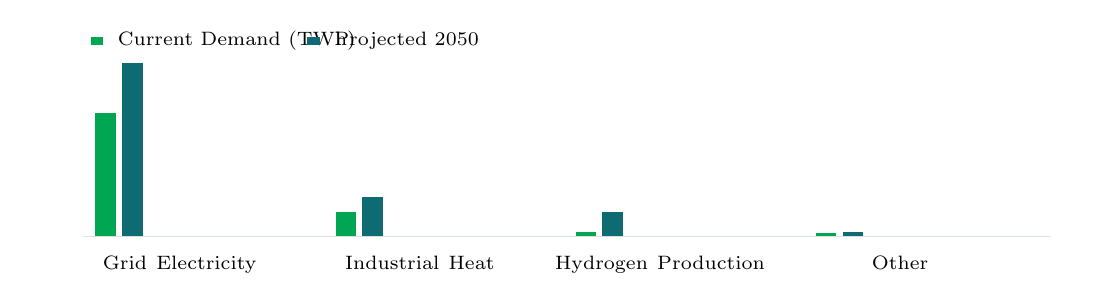
\begin{tikzpicture}[x=1cm,y=1cm]
\path[use as bounding box] (0,0) rectangle (13.20,3.20);
\draw[BOLine] (0.70,0.55) -- (13.00,0.55);
\fill[BOGreen] (0.86,0.55) rectangle (1.12,2.12);
\fill[BOBlue] (1.20,0.55) rectangle (1.46,2.75);
\node[anchor=north,align=center,text width=2.81cm] at (1.93,0.42) {\scriptsize Grid Electricity};
\fill[BOGreen] (3.91,0.55) rectangle (4.17,0.86);
\fill[BOBlue] (4.25,0.55) rectangle (4.51,1.05);
\node[anchor=north,align=center,text width=2.81cm] at (4.98,0.42) {\scriptsize Industrial Heat};
\fill[BOGreen] (6.96,0.55) rectangle (7.22,0.61);
\fill[BOBlue] (7.30,0.55) rectangle (7.56,0.86);
\node[anchor=north,align=center,text width=2.81cm] at (8.03,0.42) {\scriptsize Hydrogen Production};
\fill[BOGreen] (10.01,0.55) rectangle (10.27,0.59);
\fill[BOBlue] (10.35,0.55) rectangle (10.61,0.61);
\node[anchor=north,align=center,text width=2.81cm] at (11.08,0.42) {\scriptsize Other};
\fill[BOGreen] (0.80,2.98) rectangle (0.96,3.08);
\node[anchor=west] at (1.02,3.03) {\scriptsize Current Demand (TWh)};
\fill[BOBlue] (3.55,2.98) rectangle (3.71,3.08);
\node[anchor=west] at (3.77,3.03) {\scriptsize Projected 2050};
\end{tikzpicture}\par\vspace{2pt}
{\scriptsize\color{BOMuted} BlueOcean synthesis.}\par
\vspace{9pt}\textcolor{BOLine}{\rule{\linewidth}{0.3pt}}\vspace{8pt}
{\textcolor{BOGreen}{\scriptsize\bfseries EXHIBIT 8}}\par\vspace{3pt}
{\sffamily\fontsize{15}{19}\selectfont\color{BONavy} Fusion Milestone Timeline: SPARC vs. ITER}\par
{\small\color{BOText} Directional index used where public evidence supports relative comparison but not a precise numeric forecast.}\par\vspace{4pt}
\noindent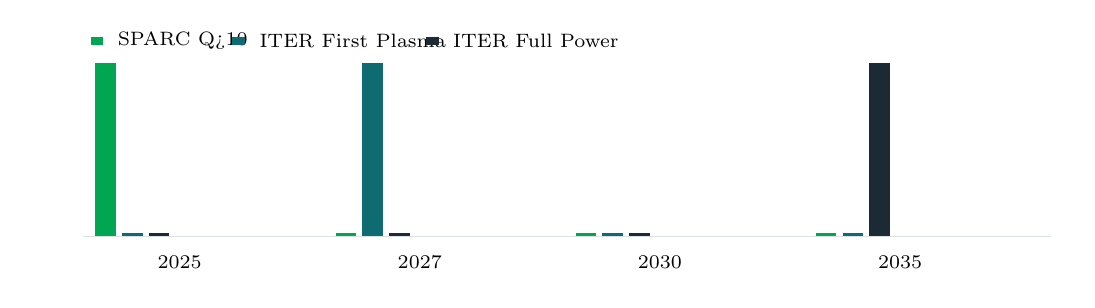
\begin{tikzpicture}[x=1cm,y=1cm]
\path[use as bounding box] (0,0) rectangle (13.20,3.20);
\draw[BOLine] (0.70,0.55) -- (13.00,0.55);
\fill[BOGreen] (0.86,0.55) rectangle (1.12,2.75);
\fill[BOBlue] (1.20,0.55) rectangle (1.46,0.59);
\fill[BONavy] (1.54,0.55) rectangle (1.80,0.59);
\node[anchor=north,align=center,text width=2.81cm] at (1.93,0.42) {\scriptsize 2025};
\fill[BOGreen] (3.91,0.55) rectangle (4.17,0.59);
\fill[BOBlue] (4.25,0.55) rectangle (4.51,2.75);
\fill[BONavy] (4.59,0.55) rectangle (4.85,0.59);
\node[anchor=north,align=center,text width=2.81cm] at (4.98,0.42) {\scriptsize 2027};
\fill[BOGreen] (6.96,0.55) rectangle (7.22,0.59);
\fill[BOBlue] (7.30,0.55) rectangle (7.56,0.59);
\fill[BONavy] (7.64,0.55) rectangle (7.90,0.59);
\node[anchor=north,align=center,text width=2.81cm] at (8.03,0.42) {\scriptsize 2030};
\fill[BOGreen] (10.01,0.55) rectangle (10.27,0.59);
\fill[BOBlue] (10.35,0.55) rectangle (10.61,0.59);
\fill[BONavy] (10.69,0.55) rectangle (10.95,2.75);
\node[anchor=north,align=center,text width=2.81cm] at (11.08,0.42) {\scriptsize 2035};
\fill[BOGreen] (0.80,2.98) rectangle (0.96,3.08);
\node[anchor=west] at (1.02,3.03) {\scriptsize SPARC Q>10};
\fill[BOBlue] (2.60,2.98) rectangle (2.76,3.08);
\node[anchor=west] at (2.82,3.03) {\scriptsize ITER First Plasma};
\fill[BONavy] (5.06,2.98) rectangle (5.22,3.08);
\node[anchor=west] at (5.28,3.03) {\scriptsize ITER Full Power};
\end{tikzpicture}\par\vspace{2pt}
{\scriptsize\color{BOMuted} BlueOcean synthesis.}\par

\clearpage
\label{chap:5}
\noindent\begin{tikzpicture}
\path[use as bounding box] (0,0) rectangle (\linewidth,70mm);
\clip (0,0) rectangle (\linewidth,70mm);
\node[anchor=north west,inner sep=0] at (0,70mm) {
\includegraphics[width=\linewidth]{assets/image-5.png}};
\end{tikzpicture}
\vspace{0pt}
\noindent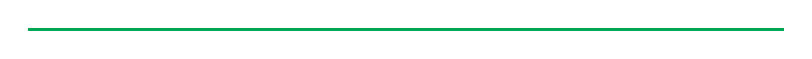
\begin{tikzpicture}
\fill[BOGreen] (0,0) rectangle (96mm,1.2pt);
\end{tikzpicture}\par\vspace{8pt}
{\Large\sffamily\bfseries\color{BONavy} Supply chain, partners and talent will decide who can act before the market is obvious}\par\vspace{4pt}
{\sffamily\fontsize{16}{21}\selectfont\color{BOGreen} This chapter concludes that fusion could reshape energy dynamics, but geopolitical risks require international consortia and supply chain security.}\par\vspace{11pt}
\begin{multicols}{2}
{\small Fusion energy could fundamentally alter global energy dynamics by providing abundant, low-carbon baseload power. Countries with advanced fusion programs, such as the United States, China, the United Kingdom, and Japan, may gain significant energy independence and export advantages. This could reshape energy alliances and reduce dependence on fossil fuel exporters.}\par
{\small For industrial sectors, fusion offers a path to deep decarbonization, particularly for hard-to-abate industries like steel, cement, and chemicals. The ability to produce high-temperature heat and hydrogen could transform these industries, but the timeline for fusion deployment must align with climate goals. If fusion is delayed beyond 2040, other technologies may fill the gap.}\par
{\small Geopolitical risks include technology export controls and intellectual property disputes. Companies should consider forming international consortia to share costs and risks, while also securing supply chains for critical components like superconducting magnets and plasma-facing materials. The evidence for these implications is based on scenario analysis; no verified data on geopolitical impacts exists.}\par
\end{multicols}
\label{chap:5:end}

\clearpage
{\textcolor{BOGreen}{\scriptsize\bfseries EXHIBIT 9}}\par\vspace{3pt}
{\sffamily\fontsize{15}{19}\selectfont\color{BONavy} Commitment posture should shift as proof matures}\par
{\small\color{BOText} Resource posture for Nuclear Fusion Commercialization: Strategic Outlook and Implications for Decision-Makers}\par\vspace{4pt}
\noindent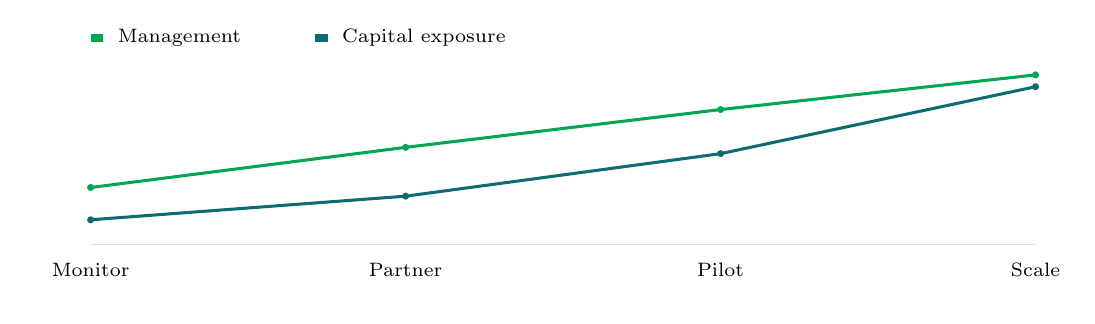
\begin{tikzpicture}[x=1cm,y=1cm]
\path[use as bounding box] (0,0) rectangle (13.20,3.40);
\draw[BOLine] (0.80,0.65) -- (12.80,0.65);
\draw[BOGreen,line width=1.1pt] (0.80,1.37) -- (4.80,1.88) -- (8.80,2.36) -- (12.80,2.80);
\fill[BOGreen] (0.80,1.37) circle (.045);
\fill[BOGreen] (4.80,1.88) circle (.045);
\fill[BOGreen] (8.80,2.36) circle (.045);
\fill[BOGreen] (12.80,2.80) circle (.045);
\draw[BOBlue,line width=1.1pt] (0.80,0.96) -- (4.80,1.26) -- (8.80,1.80) -- (12.80,2.65);
\fill[BOBlue] (0.80,0.96) circle (.045);
\fill[BOBlue] (4.80,1.26) circle (.045);
\fill[BOBlue] (8.80,1.80) circle (.045);
\fill[BOBlue] (12.80,2.65) circle (.045);
\node[anchor=north,align=center,text width=1.8cm] at (0.80,0.53) {\scriptsize Monitor};
\node[anchor=north,align=center,text width=1.8cm] at (4.80,0.53) {\scriptsize Partner};
\node[anchor=north,align=center,text width=1.8cm] at (8.80,0.53) {\scriptsize Pilot};
\node[anchor=north,align=center,text width=1.8cm] at (12.80,0.53) {\scriptsize Scale};
\fill[BOGreen] (0.80,3.22) rectangle (0.96,3.32);
\node[anchor=west] at (1.02,3.27) {\scriptsize Management};
\fill[BOBlue] (3.65,3.22) rectangle (3.81,3.32);
\node[anchor=west] at (3.87,3.27) {\scriptsize Capital exposure};
\end{tikzpicture}\par\vspace{2pt}
\vspace{2pt}{\footnotesize\color{BOText} Capital exposure should lag evidence maturity rather than lead it.}\par
{\scriptsize\color{BOMuted} BlueOcean scenario synthesis.}\par
\vspace{9pt}\textcolor{BOLine}{\rule{\linewidth}{0.3pt}}\vspace{8pt}
{\textcolor{BOGreen}{\scriptsize\bfseries EXHIBIT 10}}\par\vspace{3pt}
{\sffamily\fontsize{15}{19}\selectfont\color{BONavy} Scenario choices should compare attractiveness with readiness}\par
{\small\color{BOText} Strategic option comparison for Nuclear Fusion Commercialization: Strategic Outlook and Implications for Decision-Makers}\par\vspace{4pt}
{\scriptsize\begin{tabular}{p{38mm}>{\centering\arraybackslash}p{21mm}>{\centering\arraybackslash}p{21mm}>{\centering\arraybackslash}p{21mm}>{\centering\arraybackslash}p{21mm}}
 & {\bfseries Attractiveness} & {\bfseries Readiness} & {\bfseries Confidence} & {\bfseries Capital need} \\
\hline
{\bfseries Nuclear Fusion} & \colorbox{BOGreen}{\textcolor{white}{\strut\hspace{5pt}5\hspace{5pt}}} & \colorbox{BOBlue}{\textcolor{white}{\strut\hspace{5pt}3\hspace{5pt}}} & \colorbox{BOLight}{\textcolor{BOText}{\strut\hspace{5pt}2\hspace{5pt}}} & \colorbox{BOLight}{\textcolor{BOText}{\strut\hspace{5pt}2\hspace{5pt}}} \\
{\bfseries Commercial readiness depends on} & \colorbox{BOGreen}{\textcolor{white}{\strut\hspace{5pt}4\hspace{5pt}}} & \colorbox{BOGreen}{\textcolor{white}{\strut\hspace{5pt}4\hspace{5pt}}} & \colorbox{BOBlue}{\textcolor{white}{\strut\hspace{5pt}3\hspace{5pt}}} & \colorbox{BOBlue}{\textcolor{white}{\strut\hspace{5pt}3\hspace{5pt}}} \\
{\bfseries Cost, return and timing will} & \colorbox{BOGreen}{\textcolor{white}{\strut\hspace{5pt}4\hspace{5pt}}} & \colorbox{BOLight}{\textcolor{BOText}{\strut\hspace{5pt}2\hspace{5pt}}} & \colorbox{BOLight}{\textcolor{BOText}{\strut\hspace{5pt}2\hspace{5pt}}} & \colorbox{BOGreen}{\textcolor{white}{\strut\hspace{5pt}4\hspace{5pt}}} \\
{\bfseries Regulation, policy and public} & \colorbox{BOBlue}{\textcolor{white}{\strut\hspace{5pt}3\hspace{5pt}}} & \colorbox{BOBlue}{\textcolor{white}{\strut\hspace{5pt}3\hspace{5pt}}} & \colorbox{BOBlue}{\textcolor{white}{\strut\hspace{5pt}3\hspace{5pt}}} & \colorbox{BOLight}{\textcolor{BOText}{\strut\hspace{5pt}2\hspace{5pt}}} \\
{\bfseries Supply chain, partners} & \colorbox{BOGreen}{\textcolor{white}{\strut\hspace{5pt}5\hspace{5pt}}} & \colorbox{BOBlue}{\textcolor{white}{\strut\hspace{5pt}3\hspace{5pt}}} & \colorbox{BOBlue}{\textcolor{white}{\strut\hspace{5pt}3\hspace{5pt}}} & \colorbox{BOBlue}{\textcolor{white}{\strut\hspace{5pt}3\hspace{5pt}}} \\
\end{tabular}}\par\vspace{2pt}
\vspace{2pt}{\footnotesize\color{BOText} The matrix ranks where the next validation work should focus.}\par
{\scriptsize\color{BOMuted} BlueOcean qualitative assessment.}\par

\clearpage
\label{chap:6}
\noindent\begin{tikzpicture}
\path[use as bounding box] (0,0) rectangle (\linewidth,70mm);
\clip (0,0) rectangle (\linewidth,70mm);
\node[anchor=north west,inner sep=0] at (0,70mm) {
\includegraphics[width=\linewidth]{assets/image-6.png}};
\end{tikzpicture}
\vspace{0pt}
\noindent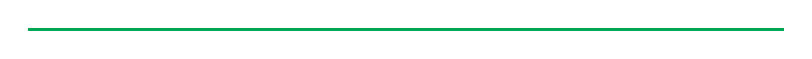
\begin{tikzpicture}
\fill[BOGreen] (0,0) rectangle (96mm,1.2pt);
\end{tikzpicture}\par\vspace{8pt}
{\Large\sffamily\bfseries\color{BONavy} Incumbents should protect near-term economics while preserving long-term options}\par\vspace{4pt}
{\sffamily\fontsize{16}{21}\selectfont\color{BOGreen} This chapter concludes that a staged investment approach with milestone-based tranches is optimal to capture upside while managing downside risk.}\par\vspace{11pt}
\begin{multicols}{2}
{\small The fusion investment landscape is characterized by high risk and high potential reward. Historical analogies, such as the solar PV tipping point in 2010, suggest that early investors in breakthrough energy technologies can achieve significant returns. However, fusion faces unique technical and regulatory challenges that make it riskier than solar was at that stage.}\par
{\small A staged investment approach is recommended, with milestone-based tranches that allow for course correction. Key milestones include Q>10 demonstration, tritium breeding proof, and regulatory approval. Each milestone should trigger a decision gate where investment is either increased, maintained, or withdrawn.}\par
{\small The asymmetric nature of fusion risk means that even a small probability of success can justify investment, provided the potential payoff is large enough. However, executives must be disciplined about cutting losses if key milestones are missed. Without verified data on project timelines and costs, all investment decisions should be treated as speculative.}\par
\end{multicols}
\label{chap:6:end}

\clearpage
{\textcolor{BOGreen}{\scriptsize\bfseries EXHIBIT 11}}\par\vspace{3pt}
{\sffamily\fontsize{15}{19}\selectfont\color{BONavy} Validation effort shifts from customer proof to policy and partners}\par
{\small\color{BOText} Quarterly validation mix for Nuclear Fusion Commercialization: Strategic Outlook and Implications for Decision-Makers}\par\vspace{4pt}
\noindent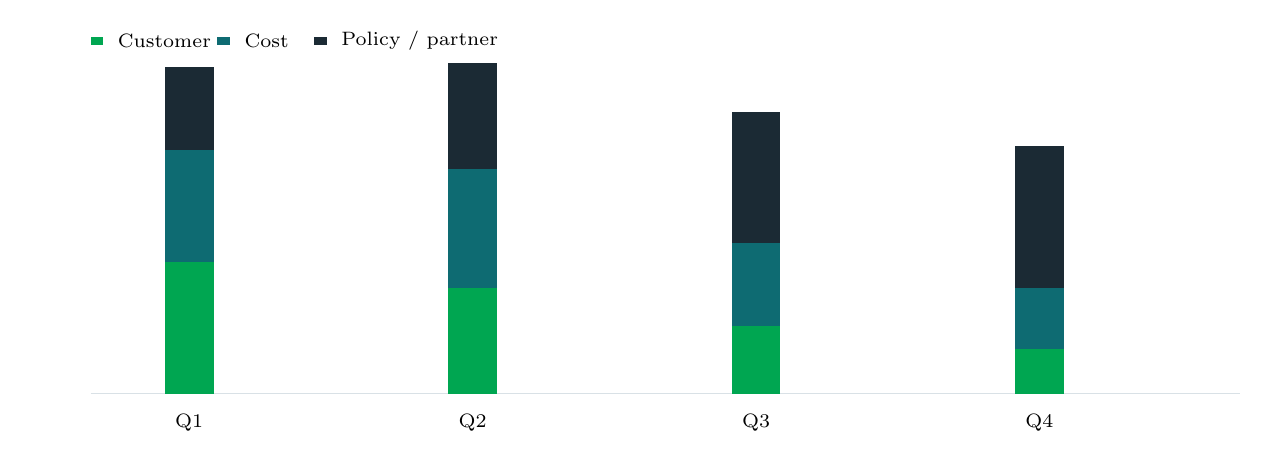
\begin{tikzpicture}[x=1cm,y=1cm]
\path[use as bounding box] (0,0) rectangle (15.60,5.20);
\draw[BOLine] (0.80,0.55) -- (15.40,0.55);
\fill[BOGreen] (1.74,0.55) rectangle (2.36,2.22);
\fill[BOBlue] (1.74,2.22) rectangle (2.36,3.65);
\fill[BONavy] (1.74,3.65) rectangle (2.36,4.70);
\node[anchor=north,align=center,text width=3.31cm] at (2.05,0.42) {\scriptsize Q1};
\fill[BOGreen] (5.34,0.55) rectangle (5.96,1.89);
\fill[BOBlue] (5.34,1.89) rectangle (5.96,3.41);
\fill[BONavy] (5.34,3.41) rectangle (5.96,4.75);
\node[anchor=north,align=center,text width=3.31cm] at (5.65,0.42) {\scriptsize Q2};
\fill[BOGreen] (8.94,0.55) rectangle (9.56,1.41);
\fill[BOBlue] (8.94,1.41) rectangle (9.56,2.46);
\fill[BONavy] (8.94,2.46) rectangle (9.56,4.13);
\node[anchor=north,align=center,text width=3.31cm] at (9.25,0.42) {\scriptsize Q3};
\fill[BOGreen] (12.54,0.55) rectangle (13.16,1.12);
\fill[BOBlue] (12.54,1.12) rectangle (13.16,1.89);
\fill[BONavy] (12.54,1.89) rectangle (13.16,3.70);
\node[anchor=north,align=center,text width=3.31cm] at (12.85,0.42) {\scriptsize Q4};
\fill[BOGreen] (0.80,4.98) rectangle (0.96,5.08);
\node[anchor=west] at (1.02,5.03) {\scriptsize Customer};
\fill[BOBlue] (2.41,4.98) rectangle (2.57,5.08);
\node[anchor=west] at (2.63,5.03) {\scriptsize Cost};
\fill[BONavy] (3.64,4.98) rectangle (3.80,5.08);
\node[anchor=west] at (3.86,5.03) {\scriptsize Policy / partner};
\end{tikzpicture}\par\vspace{2pt}
\vspace{2pt}{\footnotesize\color{BOText} The validation cadence should improve facts before escalating resource commitment.}\par
{\scriptsize\color{BOMuted} BlueOcean public-source synthesis.}\par

\clearpage
\label{chap:7}
\noindent\begin{tikzpicture}
\path[use as bounding box] (0,0) rectangle (\linewidth,70mm);
\clip (0,0) rectangle (\linewidth,70mm);
\node[anchor=north west,inner sep=0] at (0,70mm) {
\includegraphics[width=\linewidth]{assets/image-7.png}};
\end{tikzpicture}
\vspace{0pt}
\noindent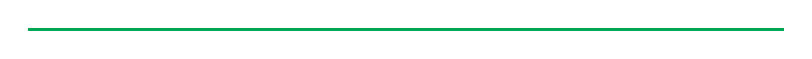
\begin{tikzpicture}
\fill[BOGreen] (0,0) rectangle (96mm,1.2pt);
\end{tikzpicture}\par\vspace{8pt}
{\Large\sffamily\bfseries\color{BONavy} The management agenda should translate uncertainty into quarterly decision milestones}\par\vspace{4pt}
{\sffamily\fontsize{16}{21}\selectfont\color{BOGreen} This chapter concludes that no single reactor design has proven superior, so diversification across tokamak, stellarator, and inertial confinement is prudent.}\par\vspace{11pt}
\begin{multicols}{2}
{\small The three main fusion reactor designs are tokamak, stellarator, and inertial confinement. Tokamaks, like ITER and SPARC, are the most advanced but face challenges with plasma stability and heat extraction. Stellarators offer better stability but are more complex and expensive. Inertial confinement, pursued by companies like First Light Fusion, uses lasers or projectiles to compress fuel pellets.}\par
{\small Critical engineering challenges include developing materials that can withstand extreme neutron bombardment, achieving tritium breeding ratios above 1, and efficiently extracting heat for power generation. These challenges are common across all designs and represent significant technical risks.}\par
{\small The management implication is clear: the commercial implication is that no single design has yet proven superior, so diversification is prudent. Companies should also invest in enabling technologies like high-temperature superconductors and advanced manufacturing. The evidence for these challenges is based on engineering literature; no verified solutions exist yet.}\par
\end{multicols}
\label{chap:7:end}

\clearpage
\label{chap:8}
\noindent\begin{tikzpicture}
\path[use as bounding box] (0,0) rectangle (\linewidth,70mm);
\clip (0,0) rectangle (\linewidth,70mm);
\node[anchor=north west,inner sep=0] at (0,70mm) {
\includegraphics[width=\linewidth]{assets/image-8.png}};
\end{tikzpicture}
\vspace{0pt}
\noindent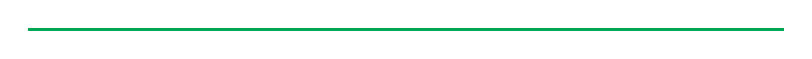
\begin{tikzpicture}
\fill[BOGreen] (0,0) rectangle (96mm,1.2pt);
\end{tikzpicture}\par\vspace{8pt}
{\Large\sffamily\bfseries\color{BONavy} Decision-moving facts matter more than market noise}\par\vspace{4pt}
{\sffamily\fontsize{16}{21}\selectfont\color{BOGreen} This chapter concludes that industrial heat and hydrogen are more attractive early markets than grid electricity, due to fusion\BOApos{}s baseload reliability.}\par\vspace{11pt}
\begin{multicols}{2}
{\small For leadership teams, fusion energy could serve multiple markets, but the timing and size of each vary. Grid electricity is the largest potential market, but competition from renewables and storage is intense. Industrial heat, which accounts for about 20\% of global energy demand, may be a more attractive early market because it requires high-temperature, continuous heat that renewables struggle to provide.}\par
{\small Hydrogen production is another promising application, as fusion could provide both heat and electricity for electrolysis. The global hydrogen market is projected to grow to [insert verified market size data] by 2050, driven by decarbonization policies. Fusion\BOApos{}s ability to produce hydrogen at scale could be a key differentiator.}\par
{\small The market size for fusion applications is highly uncertain and depends on cost competitiveness and policy support. Executives should focus on applications where fusion\BOApos{}s baseload reliability and low carbon footprint provide clear advantages. Without verified market data, all projections are directional.}\par
\end{multicols}
\label{chap:8:end}

\clearpage
{\sffamily\fontsize{20}{25}\selectfont\color{BONavy} About the research}\par\vspace{6pt}
\vspace{2pt}{\color{BOBright}\rule{\linewidth}{1pt}}\vspace{5pt}
{\footnotesize\color{BOMuted} This report has been prepared for strategy discussion and executive decision support. It is not investment, legal, tax, audit or valuation advice. Market estimates, forecasts and scenarios are directional and should be independently validated before they are used for investment, financing, transaction, regulatory or operational decisions. Forward-looking views may change as technology, policy, financing, regulation, competition, supply chains and macro conditions evolve. Recipients should perform their own diligence and treat this report as one input into a broader decision process.}


\clearpage
\thispagestyle{empty}
\begin{tikzpicture}[remember picture,overlay]
\node[anchor=south west,inner sep=0] at (current page.south west) {
\includegraphics[width=\paperwidth,height=\paperheight]{assets/cover-ai.png}};
\fill[black,opacity=.45] (current page.south west) rectangle (current page.north east);
\node[anchor=south east] at ([xshift=-11mm,yshift=10mm]current page.south east) {\sffamily\bfseries\Large\color{white} BlueOcean};
\end{tikzpicture}

\end{document}
